\documentclass[tikz,border=8pt]{standalone}
\usepackage{amsmath,amssymb,lmodern}
\usetikzlibrary{arrows.meta,positioning}
\begin{document}
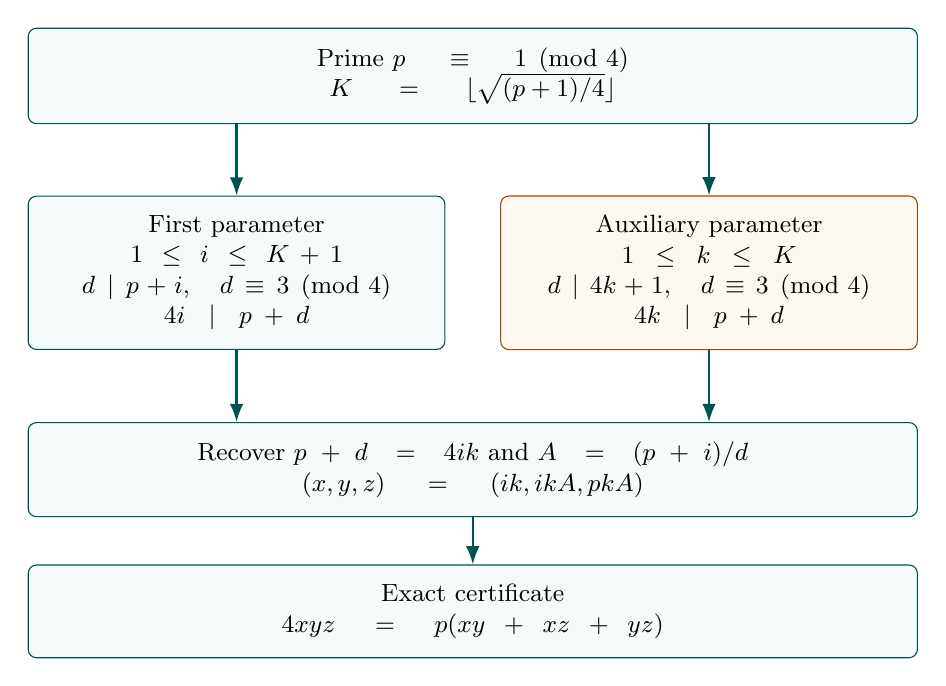
\begin{tikzpicture}[
  >=Latex,
  box/.style={draw=teal!65!black,rounded corners=3pt,fill=teal!4,
    align=center,inner sep=7pt,font=\small,text width=4.8cm},
  line/.style={->,thick,draw=teal!65!black}
]
\node[box,text width=10.8cm] (input)
  {Prime $p\equiv1\pmod4$\\
   $K=\lfloor\sqrt{(p+1)/4}\rfloor$};
\node[box] (left) at (-3,-2.5)
  {First parameter\\$1\le i\le K+1$\\
   $d\mid p+i,\quad d\equiv3\pmod4$\\$4i\mid p+d$};
\node[box,draw=orange!60!black,fill=orange!6] (right) at (3,-2.5)
  {Auxiliary parameter\\$1\le k\le K$\\
   $d\mid4k+1,\quad d\equiv3\pmod4$\\$4k\mid p+d$};
\node[box,text width=10.8cm] (identity) at (0,-5)
  {Recover $p+d=4ik$ and $A=(p+i)/d$\\
   $(x,y,z)=(ik,ikA,pkA)$};
\node[box,text width=10.8cm] (output) at (0,-6.8)
  {Exact certificate\\$4xyz=p(xy+xz+yz)$};
\draw[line] (input.south -| left.north)--(left.north);
\draw[line] (input.south -| right.north)--(right.north);
\draw[line] (left.south)--(identity.north -| left.south);
\draw[line] (right.south)--(identity.north -| right.south);
\draw[line] (identity)--(output);
\end{tikzpicture}
\end{document}
